%
%  Summary and Conclusion
% ========================
%

\chapter{Summary and Conclusion}
\label{Ch:SnC}

The aim of this thesis project was to study the performance of an optimised electron witness bunch in a proton driven plasma wakefield accelerator section.
The study was specifically aimed at Run~2 of the AWAKE experiment, scheduled after the 2019--2020 Long Shutdown~2 of the LHC, with construction planned for the shutdown period.

In Run~1 of AWAKE, which saw first beam in December 2016, the experiment sought to probe the wakefields generated by the SPS proton bunch in a $10\unit{m}$ Rubidium plasma stage.
This was done with a wide and long electron witness bunch, capable of probing the entire phase of one plasma wavelength, and a significant fraction of the radial extent of the accelerating fields.

As of the writing of this thesis, AWAKE Run~1 enters its final few months of operation.
The results of the run have been exciting, with self-modulation confirmed and studied, and $2\unit{GeV}$ accelerated electrons seen.
[Cite the new papers here.]

With an optimised experiment for the second run, it looks promising for even better results.
The work presented in this thesis has attempted to add insight into what can be expected for the next stage with a tuned electron witness bunch that can probe the accelerating structure more precisely and hopefully be accelerated to high energy while retaining low energy spread and emittance.

% ================================================================================================================================ %
\section{Results from Simulations}
\label{Sum:Sim}

The parameter scan simulation seeking to determine how much charge, and with what bunch size, could be accelerated in AWAKE Run~2 was presented in Publication~\ref{Pub:NAPAC16}.
The aim was to maximise charge and acceleration, while minimising energy spread.
The results of the scan are shown in Figure~\ref{Fig:SimA:NAPACPD}, and show that bunches with a $\sigma_z = 40-60\unit{\mu m}$ can be accelerated without too much energy spread and at a low cost of loss of final energy.
That is, the loading of the field is just enough to make it nearly flat over the length of the bunch while not lowering the average strength of the wakefield in the same region.

\begin{figure}[hbt]
    \centering
    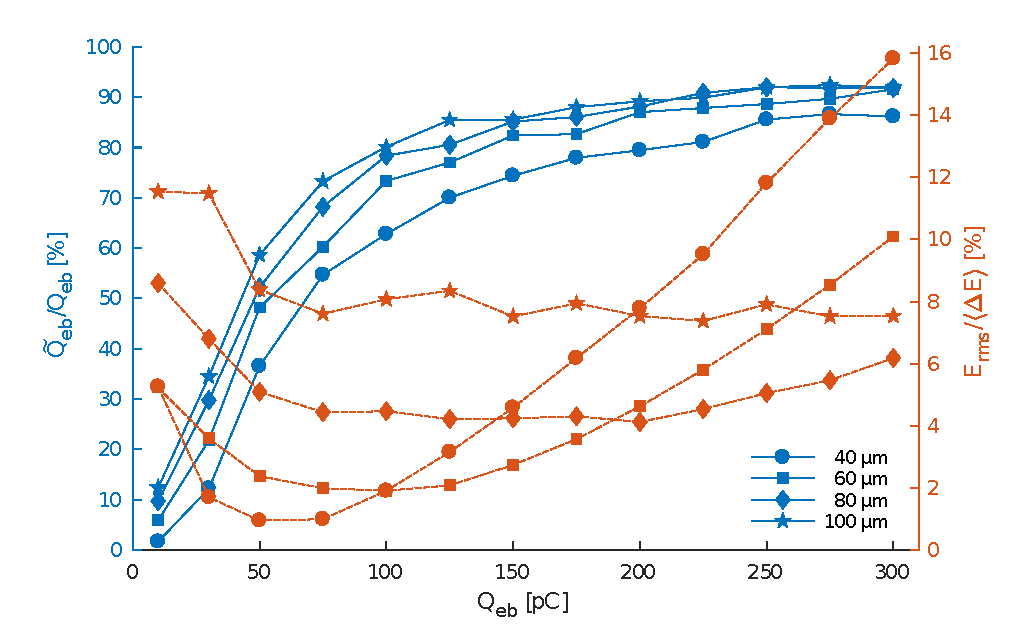
\includegraphics[width=0.8125\linewidth]{figures/BeamQuality}
    \caption{\label{Fig:Sum:BQ}
        Ratio of witness bunch charge with emittance preserved, (blue symbols, lines), as a function of initial beam charge, and relative energy spread of the accepted charge (red symbols, dashed lines), after $4\unit{m}$ of plasma and with an initial emittance of $2\unit{\mu m}$ for a range of bunch lengths.
        The figure is taken from Publication~\ref{Pub:BL17}.
    }
\end{figure}

For Publication~\ref{Pub:BL17} we switched simulation software to better understand the emittance evolution in the same range of parameters.
The main concluding results are shown in Figure~\ref{Fig:Sum:BQ}.
Again, the $\sigma_z = 40-60\unit{\mu m}$ perform well in that they flatten the accelerating wakefield without overloading it until we reach high charges, $> 150-200\unit{\mu m}$.
The different size bunches have their energy spread minima at $a\approx 50\unit{pC}$ and $a\approx 100\unit{pC}$, respectively.

Some emittance growth is inevitable due to the quasi-linear regime AWAKE operates in.
However, this growth is localised to the head of the witness bunch, while the bunch itself drives wakefields putting its own tail in the non-linear regime where no significant emittance growth occurs.
We defined a beam quality $\tilde{Q}$ to quantify this effect.
It is defined as the fraction of the bunch charge that sees a emittance growth $\leq 5\%$, laid out in Section~\ref{SimA:QTilde}.
In excess of $70\%$ of the bunch can be accelerated without any significant emittance growth, while the rest of the bunch is used to drive the non-linear region.
The simulations indicate that with these parameters, and under the assumption that the witness bunch is injected on the same axis as the drive bunch, $30-70\unit{pC}$ of electrons can be accelerated without emittance growth and with a $\lesssim 2\%$ energy spread.

Whether these conditions are reproducible in AWAKE Run~2 remains to be seen.
Alignment of the two bunches is certainly a challenge, and Publication~\ref{Pub:BL17} shows that some tolerance exists in terms of witness bunch offset, but with a cost to $\tilde{Q}$.
